\documentclass[
11pt, % The default document font size, options: 10pt, 11pt, 12pt
%codirector, % Uncomment to add a codirector to the title page
]{ProyectoVpC} 

\usepackage{enumitem}

% El títulos de la memoria, se usa en la carátula y se puede usar el cualquier lugar del documento con el comando \ttitle
\titulo{Sistema de visión por computadora para la caracterización de la altura del pasto en vías de tren}

% Nombre del posgrado, se usa en la carátula y se puede usar el cualquier lugar del documento con el comando \degreename
\posgrado{Carrera de Especialización en Sistemas Embebidos} 
%\posgrado{Carrera de Especialización en Internet de las Cosas} 
%\posgrado{Carrera de Especialización en Inteligencia Artificial}
%\posgrado{Maestría en Sistemas Embebidos} 
%\posgrado{Maestría en Internet de las cosas}

% Tu nombre, se puede usar el cualquier lugar del documento con el comando \authorname
% IMPORTANTE: no omitir titulaciones ni tildación en los nombres, también se recomienda escribir los nombres completos (tal cual los tienen en su documento)
\autor{Ing. Gustavo Ramoscelli}

% El nombre del director y co-director, se puede usar el cualquier lugar del documento con el comando \supname y \cosupname y \pertesupname y \pertecosupname
\director{Ing. Ariel Lutenberg}
\pertenenciaDirector{FIUBA} 
\codirector{} % para que aparezca en la portada se debe descomentar la opción codirector en los parámetros de documentclass
\pertenenciaCoDirector{FIUBA}

% Nombre del cliente, quien va a aprobar los resultados del proyecto, se puede usar con el comando \clientename y \empclientename
\cliente{Ing. Martín Harris}
\empresaCliente{Trenes Argentions S.A.}
 
\fechaINICIO{4 de marzo de 2025}		%Fecha de inicio de la cursada de GdP \fechaInicioName
\fechaFINALPlan{22 de abril de 2025} 	%Fecha de final de cursada de GdP
\fechaFINALTrabajo{TBD}	%Fecha de defensa pública del trabajo final


\begin{document}

\maketitle
\thispagestyle{empty}
\pagebreak


\thispagestyle{empty}
{\setlength{\parskip}{0pt}
\tableofcontents{}
}
\pagebreak


\section*{Registros de cambios}
\label{sec:registro}


\begin{table}[ht]
\label{tab:registro}
\centering
\begin{tabularx}{\linewidth}{@{}|c|X|c|@{}}
\hline
\rowcolor[HTML]{C0C0C0} 
Revisión & \multicolumn{1}{c|}{\cellcolor[HTML]{C0C0C0}Detalles de los cambios realizados} & Fecha      \\ \hline
0      & Creación del documento                                 &\fechaInicioName \\ \hline
1      & Se completa hasta el punto 5 inclusive                & 28 de marzo de 2025 \\ \hline
2      & Se completa hasta el punto 8 inclusive                & 4 de abril de 2025 \\ \hline 
%		  Se puede agregar algo más \newline
%		  En distintas líneas \newline
%		  Así                                                    & {día} de {mes} de 202X \\ \hline
%3      & Se completa hasta el punto 12 inclusive                & {día} de {mes} de 202X \\ \hline
%4      & Se completa el plan	                                 & {día} de {mes} de 202X \\ \hline

% Si hay más correcciones pasada la versión 4 también se deben especificar acá

\end{tabularx}
\end{table}

\pagebreak



\section*{Acta de constitución del proyecto}
\label{sec:acta}

\begin{flushright}
Buenos Aires, \fechaInicioName
\end{flushright}

\vspace{2cm}

Por medio de la presente se acuerda con el \authorname\hspace{1px} que su Trabajo Final de la \degreename\hspace{1px} se titulará ``\ttitle'' y consistirá en la implementación de un prototipo de un sistema de visión por computadora que genere información sobre la altura del pasto a ambos lados de las vías por donde circule una formación de tren. El trabajo tendrá un presupuesto preliminar estimado de 600 horas y un costo estimado de \$ 100.000, con fecha de inicio el \fechaInicioName\hspace{1px} y fecha de presentación pública el \fechaFinalName.

Se adjunta a esta acta la planificación inicial.

\vfill

% Esta parte se construye sola con la información que hayan cargado en el preámbulo del documento y no debe modificarla
\begin{table}[ht]
\centering
\begin{tabular}{ccc}
\begin{tabular}[c]{@{}c@{}}Dr. Ing. Ariel Lutenberg \\ Director posgrado FIUBA\end{tabular} & \hspace{2cm} & \begin{tabular}[c]{@{}c@{}}\clientename \\ \empclientename \end{tabular} \vspace{2.5cm} \\ 
\multicolumn{3}{c}{\begin{tabular}[c]{@{}c@{}} \supname \\ Director del Trabajo Final\end{tabular}} \vspace{2.5cm} \\
\end{tabular}
\end{table}




\section{1. Descripción técnica-conceptual del proyecto a realizar}
\label{sec:descripcion}

\subsection{Introducción y contexto}
\label{sec:descripcion}
El mantenimiento de la vegetación en los alrededores de las vías férreas es fundamental para garantizar la seguridad y eficiencia del transporte ferroviario. La presencia de pasto alto puede afectar la visibilidad de los maquinistas, deteriorar la infraestructura y aumentar el riesgo de incendios, especialmente en temporadas secas. Actualmente, la inspección y mantenimiento de la vegetación son tareas costosas que requieren personal capacitado y revisiones periódicas, muchas de ellas realizadas manualmente.

En este contexto, el presente proyecto propone una solución innovadora basada en inteligencia artificial (IA) y visión por computadora para automatizar el monitoreo del crecimiento de la vegetación en las vías de tren. A través de una cámara instalada en la parte frontal de una locomotora y un sistema de procesamiento de imágenes en tiempo real, se busca estimar y modelar la altura del pasto, proporcionando datos clave para la planificación del mantenimiento.

\subsection{Estado del arte y propuesta de valor}
Actualmente, las metodologías empleadas para la inspección de vegetación en el ámbito ferroviario se realizan inspecciones visuales. Esta forma de trabajo presenta limitaciones en términos de costos y accesibilidad. El uso de visión por computadora y técnicas de aprendizaje de máquina representará un avance significativo al bajar los costos que insumen las inspecciones periódicas de los trabajadores.

La propuesta de valor del sistema radica en su capacidad para operar en tiempo real, facilitando la detección y medición precisa del crecimiento del pasto sin interrumpir las operaciones ferroviarias. Este enfoque no solo optimiza la planificación de mantenimiento, sino que también reduce costos y minimiza riesgos operativos.

\subsection{Problema y solución propuesta}
El problema central que aborda este proyecto es la falta de un sistema automatizado y eficiente para el monitoreo del crecimiento del pasto en las vías ferroviarias. Actualmente, las inspecciones manuales y los mantenimientos programados pueden ser ineficientes, generando gastos innecesarios y riesgos para la infraestructura.

La solución consiste en un sistema basado en IA que emplea aprendizaje de máquina para segmentar imágenes de video y predecir la altura del pasto en tiempo real. La información generada servirá como insumo para la toma de decisiones sobre el mantenimiento de la vegetación, optimizando la asignación de recursos y mejorando la seguridad operativa.

\subsection{Descripción funcional y diagrama en bloques}
El sistema se compone de los siguientes módulos principales:

\begin{itemize}
\item{\bf Captura de Video:} Una cámara montada en la locomotora captura imágenes del entorno en diversas condiciones climáticas y de iluminación.

\item{\bf Procesamiento de Imágenes:} Se aplica segmentación basada en color y modelos de redes neuronales para identificar la vegetación.

\item{\bf Estimación de Altura:} La red neuronal entrenada analiza las imágenes y calcula la altura del pasto en cada sección de la vía.

\item{\bf Almacenamiento y Visualización:} Los datos generados se almacenan en una base de datos para su consulta y análisis.
\end{itemize}
A continuación, se presenta un diagrama en bloques del sistema:

\begin{figure}[htpb]
\centering 
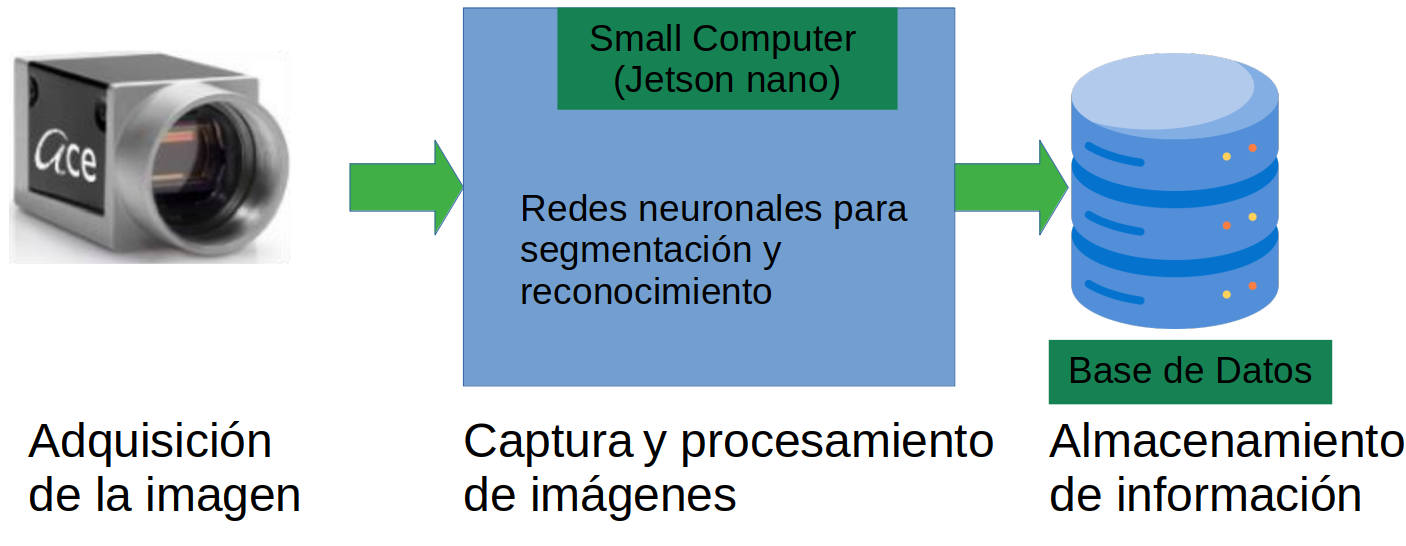
\includegraphics[width=.65\textwidth]{./Figuras/diagBloques.png}
\caption{Diagrama en bloques del sistema.}
\label{fig:diagBloques}
\end{figure}
\vspace{25px}

\subsection{Impacto y futuras aplicaciones}
Este proyecto tiene el potencial de mejorar el mantenimiento ferroviario al proporcionar un método preciso, eficiente y escalable para el monitoreo de la vegetación. En el futuro, el sistema podría integrarse con tecnologías adicionales, como sensores LiDAR que permitirán el sensado nocturno. Asimismo, su implementación en múltiples locomotoras permitiría una cobertura extensiva y una planificación de mantenimiento basada en datos en tiempo real.

\section{2. Identificación y análisis de los interesados}
\label{sec:interesados}

\begin{table}[ht]
%\caption{Identificación de los interesados}
%\label{tab:interesados}
\begin{tabularx}{\linewidth}{@{}|l|X|X|l|@{}}
\hline
\rowcolor[HTML]{C0C0C0} 
Rol           & Nombre y Apellido & Organización 	& Puesto 	\\ \hline
Auspiciante   & \clientename                  &  \empclientename            &        	\\ \hline
Cliente       & \clientename      &\empclientename	&        	\\ \hline
%Impulsor      &                   &              	&        	\\ %\hline
Responsable   & \authorname       & FIUBA        	& Alumno 	\\ \hline
%Colaboradores &                   &              	&        	\\ %\hline
Orientador    & \supname	      & \pertesupname 	& Director del Trabajo Final \\ \hline
%Equipo        & miembro1 \newline 
%				miembro2          &              	&        	\\ %\hline
%Opositores    &                   &              	&        	\\ %\hline
Usuario final & Sistemas de Mantenimiento                 & \empclientename   &        	\\ \hline
\end{tabularx}
\end{table}

\begin{itemize}
	\item Orientador: El/la \supname \ es experto/a en sistemas de visión por computadora y me asistirá en la parte de implementación y entrenamiento del modelo de redes neuronales artificiales.
	\item Auspiciante: es riguroso y exigente con la rendición de gastos. Prestar mucha atención a esto.
\end{itemize}

\section{3. Propósito del proyecto}
\label{sec:proposito}

Optimizar el monitoreo y gestión de la vegetación en vías de tren mediante un sistema automatizado de visión por computadora que permita estimar la altura del pasto en tiempo real. La solución busca mejorar la seguridad operativa, reducir costos asociados a la supervisión manual y facilitar la toma de decisiones en el mantenimiento ferroviario, proporcionando información precisa y accesible para optimizar la planificación de intervenciones.

\section{4. Alcance del proyecto}
\label{sec:alcance}

El proyecto incluye:
\begin{itemize}
\item Captura de datos mediante la instalación de una cámara en la parte frontal de una locomotora para registrar videos en diferentes condiciones climáticas y de iluminación.
\item Procesamiento de imágenes aplicando técnicas de segmentación para identificar la vegetación en los alrededores de las vías.
\item Entrenamiento de un modelo de inteligencia artificial basado en redes neuronales para estimar la altura del pasto a partir de las imágenes capturadas.
\item Validación del sistema en entornos controlados y pruebas en campo para evaluar su precisión y desempeño bajo distintas condiciones.
\item Análisis de factibilidad de procesamiento en tiempo real utilizando hardware especializado como GPU o dispositivos embebidos.
\item Desarrollo de un prototipo funcional, que permitirá demostrar la viabilidad del sistema y su potencial implementación en el sector ferroviario.

\end{itemize}
El proyecto no incluye:
\begin{itemize}
\item Implementación a gran escala en múltiples locomotoras o redes ferroviarias.
\item Integración con sensores adicionales como LiDAR o GPS, aunque se plantea como una posible extensión futura.
\item Desarrollo de una plataforma de monitoreo centralizada para la gestión de datos a nivel operativo.
\item El alcance del proyecto se limita al diseño, desarrollo y validación de un sistema experimental, proporcionando las bases para futuras mejoras e implementación en escenarios reales.
\end{itemize}

\section{5. Supuestos del proyecto}
\label{sec:supuestos}
Para el desarrollo del presente proyecto se supone que:
\begin{itemize}
\item Se contará con acceso a una locomotora de pruebas para la instalación de la cámara y la recolección de datos en distintas condiciones climáticas.
\item La capacidad de procesamiento de los equipos utilizados será suficiente para ejecutar modelos de visión por computadora en tiempo real o con una latencia aceptable.
\item Se dispondrá de un conjunto de datos representativo para entrenar y validar la red neuronal, con ejemplos en diversas condiciones de iluminación y tipos de vegetación.
\item No habrá restricciones regulatorias o normativas que impidan la instalación de equipos en la locomotora durante la fase experimental.
\item Se contará con el apoyo de personal técnico para la instalación y configuración de hardware y software necesarios para la prueba del sistema.
\item Los costos de adquisición de hardware y almacenamiento de datos serán viables dentro del presupuesto del proyecto.
\item No se prevén cambios significativos en las condiciones de operación ferroviaria que afecten el desarrollo del sistema durante la ejecución del proyecto.
\end{itemize}

\section{6. Product Backlog}
\label{sec:backlog}

El siguiente Product Backlog se organiza en cuatro épicas principales, cada una con sus historias de usuario (HU). A cada historia se le asigna una prioridad (Alta, Media o Baja), si es opcional y una estimación en Story Points (SP), calculada según dificultad, complejidad e incertidumbre. Se adopta la serie de Fibonacci para redondear el total.

\begin{itemize}
  \item \textbf{\'{E}pica 1: Captura y gestión de datos}
    \begin{itemize}
      \item \textbf{HU1:} 
      \emph{Como personal de mantenimiento, quiero instalar y configurar la cámara en la locomotora para capturar imágenes en diferentes condiciones.}
        \begin{itemize}[label=$\cdot$]
          \item Dificultad: 3
          \item Complejidad: 3
          \item Incertidumbre: 2
          \item Suma: 8 $\rightarrow$ \textbf{Story Points: 8}
          \item Prioridad: Alta
          \item Opcional: No
        \end{itemize}

      \item \textbf{HU2:} 
      \emph{Como analista de datos, quiero almacenar y organizar las imágenes en un repositorio central para su posterior procesamiento.}
        \begin{itemize}[label=$\cdot$]
          \item Dificultad: 3
          \item Complejidad: 4
          \item Incertidumbre: 3
          \item Suma: 10 $\rightarrow$ \textbf{Story Points: 13}
          \item Prioridad: Alta
          \item Opcional: No
        \end{itemize}
    \end{itemize}

  \item \textbf{\'{E}pica 2: Entrenamiento y validación del modelo de IA}
    \begin{itemize}
      \item \textbf{HU3:}
      \emph{Como ingeniero de software embebido, quiero entrenar un modelo de redes neuronales para estimar la altura del pasto con precisión.}
        \begin{itemize}[label=$\cdot$]
          \item Dificultad: 5
          \item Complejidad: 5
          \item Incertidumbre: 3
          \item Suma: 13 $\rightarrow$ \textbf{Story Points: 13}
          \item Prioridad: Alta
          \item Opcional: No
        \end{itemize}

      \item \textbf{HU4:}
      \emph{Como responsable de calidad, quiero validar el modelo en pruebas de campo para asegurar un desempeño confiable.}
        \begin{itemize}[label=$\cdot$]
          \item Dificultad: 4
          \item Complejidad: 4
          \item Incertidumbre: 3
          \item Suma: 11 $\rightarrow$ \textbf{Story Points: 13}
          \item Prioridad: Media
          \item Opcional: No
        \end{itemize}
    \end{itemize}

  \item \textbf{\'{E}pica 3: Visualización de información y alertas}
    \begin{itemize}
      \item \textbf{HU5:}
      \emph{Como personal de mantenimiento, quiero ver en tiempo real la estimación de la altura del pasto para planificar intervenciones.}
        \begin{itemize}[label=$\cdot$]
          \item Dificultad: 3
          \item Complejidad: 3
          \item Incertidumbre: 3
          \item Suma: 9 $\rightarrow$ \textbf{Story Points: 13}
          \item Prioridad: Alta
          \item Opcional: No
        \end{itemize}

      \item \textbf{HU6:}
      \emph{Como jefe de operaciones, quiero recibir alertas automáticas cuando el pasto supere un umbral crítico para coordinar acciones preventivas.}
        \begin{itemize}[label=$\cdot$]
          \item Dificultad: 3
          \item Complejidad: 2
          \item Incertidumbre: 3
          \item Suma: 8 $\rightarrow$ \textbf{Story Points: 8}
          \item Prioridad: Alta
          \item Opcional: No
        \end{itemize}
    \end{itemize}

  \item \textbf{\'{E}pica 4: Gestión de acceso y confiabilidad del sistema}
    \begin{itemize}
      \item \textbf{HU7:}
      \emph{Como administrador del sistema, quiero gestionar los permisos de cada usuario para asegurar la confidencialidad de los datos.}
        \begin{itemize}[label=$\cdot$]
          \item Dificultad: 3
          \item Complejidad: 2
          \item Incertidumbre: 2
          \item Suma: 7 $\rightarrow$ \textbf{Story Points: 8}
          \item Prioridad: Media
          \item Opcional: No
        \end{itemize}

      \item \textbf{HU8:}
      \emph{Como auditor externo, quiero acceder a un historial de modificaciones y accesos para cumplir con la normativa y asegurar trazabilidad.}
        \begin{itemize}[label=$\cdot$]
          \item Dificultad: 3
          \item Complejidad: 3
          \item Incertidumbre: 3
          \item Suma: 9 $\rightarrow$ \textbf{Story Points: 13}
          \item Prioridad: Media
          \item Opcional: Sí
        \end{itemize}
    \end{itemize}
\end{itemize}


\section{7. Criterios de aceptación de historias de usuario}
\label{sec:criteriosAceptacion}

\begin{itemize}
  % ÉPICA 1
  \item \textbf{\'{E}pica 1: Captura y gestión de datos}
    \begin{itemize}
      \item \textbf{Criterios de aceptación HU1 (Instalar y configurar la cámara)}
        \begin{itemize}
          \item La cámara graba video continuo bajo condiciones diurnas, nocturnas y de clima adverso sin interrupciones.
          \item La tasa de captura (FPS) cumple el mínimo de 30\,FPS.
          \item Se validan la transmisión y el almacenamiento de video en el repositorio central sin pérdida de datos.
        \end{itemize}

      \item \textbf{Criterios de aceptación HU2 (Almacenar y organizar las imágenes)}
        \begin{itemize}
          \item Cada imagen se registra con metadatos (fecha, hora, posible ubicación) y se puede buscar en menos de 5\,segundos.
          \item Se verifica la integridad de los archivos (por ejemplo, usando checksums).
          \item El sistema maneja volúmenes de datos de al menos 1.000 imágenes/día sin fallas.
        \end{itemize}
    \end{itemize}

  % ÉPICA 2
  \item \textbf{\'{E}pica 2: Entrenamiento y validación del modelo de IA}
    \begin{itemize}
      \item \textbf{Criterios de aceptación HU3 (Entrenar el modelo de redes neuronales)}
        \begin{itemize}
          \item El modelo se entrena con más de 1.000 muestras y alcanza al menos un 85\% de exactitud (\emph{accuracy}) en pruebas internas.
          \item El proceso de entrenamiento no supera 2\,horas con la infraestructura disponible.
          \item Se generan logs y gráficas de la evolución del entrenamiento (\emph{loss}, \emph{accuracy}).
          \item El conjunto de datos de entrenamiento incluye ejemplos con distintas condiciones de iluminación (mañana, mediodía, tarde).
          \item Se documentan los hiperparámetros más relevantes (tasa de aprendizaje, número de épocas, tamaño de lote, etc.) para replicar el proceso.
        \end{itemize}

      \item \textbf{Criterios de aceptación HU4 (Validar el modelo en pruebas de campo)}
        \begin{itemize}
          \item El error promedio en la estimación de altura no supera $\pm10\%$ frente a mediciones manuales.
          \item Se comprueba un rendimiento estable ($\pm5\%$) en condiciones de iluminación variadas (mañana, mediodía, tarde).
          \item El sistema produce un informe comparativo con resultados y conclusiones de la validación.
        \end{itemize}
    \end{itemize}

  % ÉPICA 3
  \item \textbf{\'{E}pica 3: Visualización de información y alertas}
    \begin{itemize}
      \item \textbf{Criterios de aceptación HU5 (Visualizar en tiempo real la estimación de la altura)}
        \begin{itemize}
          \item El panel (dashboard) se actualiza cada minuto con la altura promedio estimada por tramo.
          \item La interfaz es intuitiva y no requiere más de 2 clics para llegar a la vista detallada de cada tramo.
          \item Se permite exportar los datos en formato PDF, con fecha/hora y alturas estimadas.
        \end{itemize}

      \item \textbf{Criterios de aceptación HU6 (Recibir alertas automáticas)}
        \begin{itemize}
          \item El usuario configura el umbral (en cm) y el sistema dispara una alerta visual y sonora al superarlo.
          \item Se envía un correo electrónico a los roles de “Jefe de Operaciones” cuando haya 5 tramos consecutivos con altura mayor al umbral.
          \item Se registra un log con fecha, hora y coordenadas aproximadas de cada alerta.
          \item Las alertas pueden configurarse para diferentes umbrales según el tipo de vía (urbana, rural, etc.).
        \end{itemize}
    \end{itemize}

  % ÉPICA 4
  \item \textbf{\'{E}pica 4: Gestión de acceso y confiabilidad del sistema}
    \begin{itemize}
      \item \textbf{Criterios de aceptación HU7 (Gestionar permisos de usuarios)}
        \begin{itemize}
          \item Existen roles (administrador, analista, mantenimiento, auditor) con privilegios claramente diferenciados.
          \item El acceso requiere usuario y contraseña, con posibilidad de habilitar doble factor de autenticación.
          \item Se registra en bitácora cada evento de creación o modificación de usuarios y roles.
        \end{itemize}

      \item \textbf{Criterios de aceptación HU8 (Historial de modificaciones y accesos)}
        \begin{itemize}
          \item Se registra en un historial inalterable (fecha, hora, usuario y cambio realizado).
          \item El filtrado por usuario, fecha y tipo de cambio no supera 5\,segundos de tiempo de respuesta.
          \item La exportación de registros se hace en CSV o PDF, conservando toda la trazabilidad.
        \end{itemize}
    \end{itemize}
\end{itemize}

\section{8. Fases de CRISP-DM}

\subsection{Comprensión del negocio}
\begin{itemize}
  \item \textbf{Objetivo:} Desarrollar un sistema de visión por computadora capaz de estimar la altura del pasto en los alrededores de las vías, reduciendo así la necesidad de inspecciones manuales y optimizando los costos y tiempos de mantenimiento.
  \item \textbf{Impacto esperado:} 
    \begin{itemize}
      \item Mejorar la seguridad operacional ferroviaria al prevenir que la vegetación alta obstruya la visibilidad o dañe la infraestructura.
      \item Optimizar recursos de mantenimiento, evitando inspecciones excesivas o tardías.
      \item Reducir costos relacionados con trabajos manuales y riesgos en campo.
    \end{itemize}
  \item \textbf{Métricas de éxito:} 
    \begin{itemize}
      \item Margen de error en la estimación de altura no mayor a un $\pm10\%$ frente a mediciones manuales de referencia.
      \item Tasa de cobertura de vías escaneadas (porcentaje de vía supervisada).
      \item Aumento en la eficiencia de planificación de corte o poda (reducción del número de inspecciones manuales realizadas).
    \end{itemize}
\end{itemize}

\subsection{Comprensión de los datos}
\begin{itemize}
  \item \textbf{Tipo de datos:} 
    \begin{itemize}
      \item Imágenes y/o video capturados desde una cámara frontal instalada en la locomotora.
      \item Posible información de telemetría asociada (fecha, hora, ubicación aproximada).
    \end{itemize}
  \item \textbf{Origen y cantidad:} 
    \begin{itemize}
      \item Se estima recolectar datos de distintas rutas ferroviarias, pudiendo alcanzar 10\,000--20\,000 fotogramas (o más), abarcando diferentes condiciones de iluminación y clima.
    \end{itemize}
  \item \textbf{Calidad de los datos:}
    \begin{itemize}
      \item Variaciones en la iluminación (día, noche, nublado).
      \item Potenciales oclusiones (objetos en el entorno).
      \item Resolución de la cámara y estabilidad de la captura (vibraciones de la locomotora).
    \end{itemize}
\end{itemize}

\subsection{Preparación de los datos}
\begin{itemize}
  \item \textbf{Selección y etiquetado:}
    \begin{itemize}
      \item Identificar fotogramas relevantes donde se visualice claramente la vegetación.
      \item Etiquetar manualmente la altura del pasto en un subconjunto de imágenes para usarlas como \emph{ground truth}.
    \end{itemize}
  \item \textbf{Procesamiento y limpieza:}
    \begin{itemize}
      \item Conversión de formatos, recortes para centrar la zona de las vías.
      \item Corrección de imágenes con baja iluminación o exceso de brillo.
      \item Normalización de tamaños (por ejemplo, 720p o 1080p) para uniformar el dataset.
    \end{itemize}
  \item \textbf{Generación de \emph{features}:}
    \begin{itemize}
      \item Segmentación de la vegetación (técnicas de \emph{color thresholding} o redes neuronales especializadas).
      \item Extracción de rasgos como textura, color o altura aproximada basada en la perspectiva de la imagen.
    \end{itemize}
\end{itemize}

\subsection{Modelado}
\begin{itemize}
  \item \textbf{Tipo de problema:} 
    \begin{itemize}
      \item Estimación de una variable continua (altura del pasto en centímetros o rangos de altura).
      \item Puede abordarse como un problema de regresión (redes neuronales convolucionales, \emph{CNN}, o modelos de visión por computadora).
    \end{itemize}
  \item \textbf{Algoritmos y modelos posibles:}
    \begin{itemize}
      \item Modelos de \emph{Deep Learning} (por ej. U-Net, FCN) para segmentar el pasto y estimar su altura.
      \item Otras redes neuronales o métodos basados en \emph{transfer learning} (ej. ResNet, VGG).
    \end{itemize}
  \item \textbf{Herramientas:}
    \begin{itemize}
      \item Bibliotecas como OpenCV, TensorFlow o PyTorch.
      \item Hardware GPU o dispositivos embebidos con aceleración (NVIDIA Jetson, Google Coral, etc.).
    \end{itemize}
\end{itemize}

\subsection{Evaluación del modelo}
\begin{itemize}
  \item \textbf{Métricas de rendimiento:}
    \begin{itemize}
      \item Error medio absoluto (MAE) o Error cuadrático medio (MSE) en la estimación de la altura.
      \item Exactitud (\emph{accuracy}) en rangos de altura (por ejemplo, si la altura es mayor a cierto umbral).
    \end{itemize}
  \item \textbf{Validación en campo:}
    \begin{itemize}
      \item Comparación de la altura estimada vs. mediciones manuales en distintos tramos de vía.
      \item Pruebas en condiciones de iluminación variadas para garantizar robustez.
    \end{itemize}
  \item \textbf{Resultados esperados:}
    \begin{itemize}
      \item Margen de error aceptable (ej. $\pm 10\%$).
      \item Informe de validación con estadísticas y gráficas comparativas.
    \end{itemize}
\end{itemize}

\subsection{Despliegue del modelo (opcional)}
\begin{itemize}
  \item \textbf{Tipo de despliegue:} 
    \begin{itemize}
      \item Integración con el prototipo de la locomotora para un procesado casi en tiempo real.
      \item Servidor local o nube (si se requiere procesar grandes volúmenes de imágenes fuera de la locomotora).
    \end{itemize}
  \item \textbf{Herramientas:} 
    \begin{itemize}
      \item Contenedores Docker para simplificar la instalación y el despliegue en diferentes equipos.
      \item Monitoreo y mantenimiento del modelo con herramientas como MLflow (opcional según alcance).
    \end{itemize}
  \item \textbf{Consideraciones futuras:}
    \begin{itemize}
      \item Posible integración con sensores adicionales (LiDAR) para mejorar la medición nocturna.
      \item Ampliación a múltiples locomotoras de la flota ferroviaria.
    \end{itemize}
\end{itemize}

\section{9. Desglose del trabajo en tareas}
\label{sec:wbs}

A partir de cada HU, descomponer en tareas concretas, técnicas y medibles:

\begin{itemize}
  \item Duración estimada: entre 2 y 8 h. Evitar tareas genéricas.
  \item Si una tarea excede 8 h, dividirla.
  \item Indicar prioridad relativa (Alta, Media, Baja).
\end{itemize}

\begin{table}[htpb]
\centering
\begin{tabularx}{\linewidth}{@{}|X|X|c|c|@{}}
\hline
\rowcolor[HTML]{C0C0C0}
Historia de usuario & Tarea técnica & Estimación & Prioridad \\ \hline
HU1 & Tarea 1 HU1 & 6 h & Alta \\ \hline
HU1 & Tarea 2 HU1 & 8 h & Alta \\ \hline
HU2 & Tarea 1 HU2 & 5 h & Media \\ \hline
HU2 & Tarea 2 HU2 & 6 h & Alta \\ \hline
... & ... & ... & ... \\ \hline
\end{tabularx}
\end{table}

\textbf{Criterios para estimar tiempos:}
\begin{itemize}
  \item Considerar dificultad, complejidad técnica y grado de incertidumbre de cada tarea.
  \item Evitar subestimar el esfuerzo requerido. Si una tarea supera las 8 h, dividirla en subtareas.
  \item Basar la estimación en la experiencia propia o en referencias de tareas similares.
\end{itemize}

\textbf{Sobre la prioridad:}
\begin{itemize}
  \item Asignar una prioridad relativa (Alta, Media o Baja) según la relevancia funcional de la tarea y su impacto en los entregables.
  \item Priorizar tareas que estén vinculadas a criterios de aceptación de las HU o que sean necesarias para desbloquear otras.
  \item Incluir tareas opcionales solo si están bien justificadas.
\end{itemize}

\textbf{Recomendaciones generales:}
\begin{itemize}
  \item Incluir al menos dos tareas por historia de usuario.
  \item El total estimado debe ser coherente con la planificación global de unas 600 horas (la cantidad de horas sugeridas para un trabajo de posgrado).
  \item Este desglose se utilizará en las secciones siguientes para armar el diagrama de Gantt (sección 10) y la planificación de sprints (sección 11).
  \item Recordar que la calidad del desglose impacta directamente en la calidad de la planificación del proyecto.
\end{itemize}


\section{10. Diagrama de Gantt}
\label{sec:gantt}

El diagrama de Gantt debe representar de forma visual y cronológica todas las tareas del proyecto, abarcando aproximadamente 600 horas totales, de las cuales entre 480 y 500 deben destinarse a tareas técnicas (desarrollo, pruebas, implementación) y entre 100 y 120 a tareas no técnicas (planificación, documentación, escritura de memoria y preparación de la defensa).

\textbf{Consignas y recomendaciones:}
\begin{itemize}
  \item Incluir tanto tareas técnicas derivadas de las HU como tareas no técnicas generales del proyecto.
  \item El eje vertical debe listar las tareas y el eje horizontal representar el tiempo en semanas o fechas.
  \item Utilizar colores diferenciados para distinguir tareas técnicas y no técnicas.
  \item Las tareas deben estar ordenadas cronológicamente y reflejar todo el ciclo del proyecto.
  \item Iniciar con la planificación del proyecto (coincidente con el inicio de Gestión de Proyectos) y finalizar con la defensa, próxima a la fecha de cierre del trabajo.
  \item Configurar el software para mostrar los códigos del desglose de tareas y los nombres junto a cada barra.
  \item Asegurarse de que la fecha final coincida con la del Acta Constitutiva.
  \item Evitar tareas genéricas o ambiguas y asegurar una secuencia lógica y realista.
  \item Las fechas pueden ser aproximadas; ajustar el ancho del diagrama según el texto y el parámetro \texttt{x unit}. Para mejorar la apariencia del diagrama, es necesario ajustar este valor y, quizás, acortar los nombres de las tareas.
\end{itemize}

\textbf{Herramientas sugeridas:}
\begin{itemize}
  \item Planner, GanttProject, Trello + plugins\\
  \url{https://blog.trello.com/es/diagrama-de-gantt-de-un-proyecto}
  \item Creately (colaborativa online)\\
  \url{https://creately.com/diagram/example/ieb3p3ml/LaTeX}
  \item LaTeX con \texttt{pgfgantt}:\\
  \url{http://ctan.dcc.uchile.cl/graphics/pgf/contrib/pgfgantt/pgfgantt.pdf}
\end{itemize}

Incluir una imagen legible del diagrama de Gantt. Si es muy ancho, presentar primero la tabla y luego el gráfico de barras.

\section{11. Planificación de Sprints}

Organizar las tareas técnicas del proyecto en sprints de trabajo que permitan distribuir de forma equilibrada la carga horaria total, estimada en 600 horas.

\textbf{Consigna:}
\begin{itemize}
  \item Completar una tabla que relacione sprints con HU y tareas técnicas correspondientes.
  \item Incluir estimación en horas para cada tarea.
  \item Indicar responsable y porcentaje de avance estimado o completado.
  \item Contemplar también tareas de planificación, documentación, redacción de memoria y preparación de defensa.
\end{itemize}

\textbf{Conceptos clave:}
\begin{itemize}
  \item Una \'{e}pica es una unidad funcional amplia; una historia de usuario es una funcionalidad concreta; un sprint es una unidad de tiempo donde se ejecutan tareas.
  \item Las tareas son el nivel más desagregado: permiten estimar tiempos, asignar responsables y monitorear progreso.
\end{itemize}

\textbf{Duración sugerida:}
\begin{itemize}
  \item Para un proyecto de 600 h, se recomienda planificar entre 10 y 12 sprints de aproximadamente 2 semanas cada uno.
  \item Asignar entre 45 y 50 horas efectivas por sprint a tareas técnicas.
  \item Reservar 100 a 120 h para actividades no técnicas (planificación, escritura, reuniones, defensa).
\end{itemize}

\textbf{Importante:}
\begin{itemize}
  \item En proyectos individuales, el responsable suele ser el propio autor.
  \item Aun así, desagregar tareas facilita el seguimiento y mejora continua.
\end{itemize}

\textbf{Conversión opcional de Story Points a horas:}
\begin{itemize}
  \item 1 SP \(\approx\) 2 h como referencia flexible.
  \item Tener en cuenta aproximaciones tipo Fibonacci.
\end{itemize}

\begin{table}[htpb]
\centering
\caption{Formato sugerido}
\begin{tabularx}{\linewidth}{@{}|l|l|X|c|l|c|@{}}
\hline
\rowcolor[HTML]{C0C0C0}
Sprint & HU o fase & Tarea & Horas / SP & Responsable & \% Completado \\ \hline
Sprint 0 & Planificación & Definir alcance y cronograma & 10 h & Alumno & 100\% \\ \hline
Sprint 0 & Planificación & Reunión con tutor/cliente & 5 h & Alumno & 50\% \\ \hline
Sprint 0 & Planificación & Ajuste de entregables & 6 h & Alumno & 25\% \\ \hline
Sprint 1 & HU1 & Tarea 1 HU1 & 6 h / 3 SP & Alumno & 0\% \\ \hline
Sprint 1 & HU1 & Tarea 2 HU1 & 10 h / 5 SP & Alumno & 0\% \\ \hline
Sprint 2 & HU2 & Tarea 1 HU2 & 7 h / 5 SP & Alumno & 0\% \\ \hline
... & ... & ... & ... & ... & ... \\ \hline
Sprint 5 & Escritura & Redacción memoria & 50 h / 34 SP & Alumno & 0\% \\ \hline
Sprint 6 & Defensa & Preparación exposición & 20 h / 13 SP & Alumno & 0\% \\ \hline
\end{tabularx}
\end{table}

\textbf{Recomendaciones:}
\begin{itemize}
  \item Verificar que la carga horaria por sprint sea equilibrada.
  \item Usar sprints de 1 a 3 semanas, acordes al cronograma general.
  \item Actualizar el \% completado durante el seguimiento del proyecto.
  \item Considerar un sprint final exclusivo para pruebas, revisión y ajustes antes de la defensa.
\end{itemize}


\section{12. Normativa y cumplimiento de datos (gobernanza)}

En esta sección se debe analizar si los datos utilizados en el proyecto están sujetos a normativas de protección de datos y privacidad, y en qué condiciones se pueden emplear.

\textbf{Aspectos a considerar:}
\begin{itemize}
  \item Evaluar si los datos están regulados por normativas como GDPR, Ley 25.326 de Protección de Datos Personales en Argentina, HIPAA u otras según jurisdicción y temática.
  \item Determinar si el uso de los datos requiere consentimiento explícito de los usuarios involucrados.
  \item Indicar si existen restricciones legales, técnicas o contractuales sobre el uso, compartición o publicación de los datos.
  \item Aclarar si los datos provienen de fuentes licenciadas, de acceso público o bajo algún tipo de autorización especial.
  \item Analizar la viabilidad del proyecto desde el punto de vista legal y ético, considerando la gobernanza de los datos.
\end{itemize}

Este análisis es clave para garantizar el cumplimiento normativo y evitar conflictos legales durante el desarrollo y publicación del proyecto.


\section{13. Gestión de riesgos}
\label{sec:riesgos}

\begin{consigna}{red}
a) Identificación de los riesgos (al menos cinco) y estimación de sus consecuencias:
 
Riesgo 1: detallar el riesgo (riesgo es algo que si ocurre altera los planes previstos de forma negativa)
\begin{itemize}
	\item Severidad (S): mientras más severo, más alto es el número (usar números del 1 al 10).\\
	Justificar el motivo por el cual se asigna determinado número de severidad (S).
	\item Probabilidad de ocurrencia (O): mientras más probable, más alto es el número (usar del 1 al 10).\\
	Justificar el motivo por el cual se asigna determinado número de (O). 
\end{itemize}   

Riesgo 2:
\begin{itemize}
	\item Severidad (S): X.\\
	Justificación...
	\item Ocurrencia (O): Y.\\
	Justificación...
\end{itemize}

Riesgo 3:
\begin{itemize}
	\item Severidad (S):  X.\\
	Justificación...
	\item Ocurrencia (O): Y.\\
	Justificación...
\end{itemize}


b) Tabla de gestión de riesgos:      (El RPN se calcula como RPN=SxO)

\begin{table}[htpb]
\centering
\begin{tabularx}{\linewidth}{@{}|X|c|c|c|c|c|c|@{}}
\hline
\rowcolor[HTML]{C0C0C0} 
Riesgo & S & O & RPN & S* & O* & RPN* \\ \hline
       &   &   &     &    &    &      \\ \hline
       &   &   &     &    &    &      \\ \hline
       &   &   &     &    &    &      \\ \hline
       &   &   &     &    &    &      \\ \hline
       &   &   &     &    &    &      \\ \hline
\end{tabularx}%
\end{table}

Criterio adoptado: 

Se tomarán medidas de mitigación en los riesgos cuyos números de RPN sean mayores a...

Nota: los valores marcados con (*) en la tabla corresponden luego de haber aplicado la mitigación.

c) Plan de mitigación de los riesgos que originalmente excedían el RPN máximo establecido:
 
Riesgo 1: plan de mitigación (si por el RPN fuera necesario elaborar un plan de mitigación).
  Nueva asignación de S y O, con su respectiva justificación:
  \begin{itemize}
	\item Severidad (S*): mientras más severo, más alto es el número (usar números del 1 al 10).
          Justificar el motivo por el cual se asigna determinado número de severidad (S).
	\item Probabilidad de ocurrencia (O*): mientras más probable, más alto es el número (usar del 1 al 10).
          Justificar el motivo por el cual se asigna determinado número de (O).
	\end{itemize}

Riesgo 2: plan de mitigación (si por el RPN fuera necesario elaborar un plan de mitigación).
 
Riesgo 3: plan de mitigación (si por el RPN fuera necesario elaborar un plan de mitigación).

\end{consigna}


\section{14. Gestión de la calidad}
\label{sec:calidad}

\begin{consigna}{red}
Elija al menos diez requerimientos que a su criterio sean los más importantes/críticos/que aportan más valor y para cada uno de ellos indique las acciones de verificación y validación que permitan asegurar su cumplimiento.

\begin{itemize} 
\item Req \#1: copiar acá el requerimiento con su correspondiente número.

\begin{itemize}
	\item Verificación para confirmar si se cumplió con lo requerido antes de mostrar el sistema al cliente. Detallar.
	\item Validación con el cliente para confirmar que está de acuerdo en que se cumplió con lo requerido. Detallar. 
\end{itemize}

\end{itemize}

Tener en cuenta que en este contexto se pueden mencionar simulaciones, cálculos, revisión de hojas de datos, consulta con expertos, mediciones, etc.  

Las acciones de verificación suelen considerar al entregable como ``caja blanca'', es decir se conoce en profundidad su funcionamiento interno.  

En cambio, las acciones de validación suelen considerar al entregable como ``caja negra'', es decir, que no se conocen los detalles de su funcionamiento interno.

\end{consigna}

\section{15. Procesos de cierre}    
\label{sec:cierre}

\begin{consigna}{red}
Establecer las pautas de trabajo para realizar una reunión final de evaluación del proyecto, tal que contemple las siguientes actividades:

\begin{itemize}
	\item Pautas de trabajo que se seguirán para analizar si se respetó el Plan de Proyecto original:\\
	 - Indicar quién se ocupará de hacer esto y cuál será el procedimiento a aplicar. 
	\item Identificación de las técnicas y procedimientos útiles e inútiles que se emplearon, los problemas que surgieron y cómo se solucionaron:\\
	 - Indicar quién se ocupará de hacer esto y cuál será el procedimiento para dejar registro.
	\item Indicar quién organizará el acto de agradecimiento a todos los interesados, y en especial al equipo de trabajo y colaboradores:\\
	  - Indicar esto y quién financiará los gastos correspondientes.
\end{itemize}

\end{consigna}

\end{document}